\chapter{Grundlagenteil}
\label{grundlagen}

Dieses Kapitel erläutert die zentralen Begriffe und Konzepte, die für die Entwicklung des \ac{KI}-basierten Chatbots von Relevanz sind. 
Ziel ist es, ein grundlegendes Verständnis für die zugrunde liegende Technologie und die verwendeten Ansätze zu schaffen und so die theoretischen Rahmenbedingungen für die nachfolgende Konzeption und Umsetzung des Chatbots zu legen.

\section{Künstliche Intelligenz}

Künstliche Intelligenz (\ac{KI}) kann zum einen als die Fähigkeit von Computersystemen verstanden werden, Aufgaben zu erledigen, die normalerweise menschliche Kognition erfordern würden (\cite[S. 406]{Sarferaz2023}). 
Zum anderen wird \ac{KI} auch als die Entwicklung intelligenter Agenten beschrieben, die in der Lage sind, ihre Umgebung zu analysieren und auf Grundlage dieser Informationen zielgerichtet zu handeln (\cite[S. 183]{Coleman2021}).
Zusammenfassend lässt sich sagen, dass beide Definitionen die Fähigkeit von \ac{KI} betonen, kognitive Funktionen des menschlichen Denkens zu simulieren, um komplexe Aufgaben zu lösen. 
Für diese Arbeit wird daher eine Definition von \ac{KI} herangezogen, die sowohl das Lernen aus Erfahrungen als auch das zielgerichtete Handeln und Lösen komplexer Probleme einschließt. (\cite[S. 183]{Coleman2021})

In dieser Arbeit wird der Fokus auf spezifische Teilbereiche der \ac{KI} gelegt, die für die Entwicklung eines Chatbots von Bedeutung sind. Dazu zählen \ac{NLP} und das \ac{ML}, 
da sie die wesentlichen Grundlagen für die Interaktion des Chatbots mit Nutzern bilden. In Abbildung \ref{fig:areas_ki} sind die in dieser Arbeit relevanten Unterbereiche der \ac{KI} dargestellt, 
wobei das \ac{ML} und das \ac{NLP} als miteinander verbundene Kerntechnologien hervorgehoben werden.

Ein weiterer zentraler Bestandteil ist das Deep Learning, eine spezialisierte Methode des maschinellen Lernens, die es ermöglicht, Muster und komplexe Zusammenhänge in großen Datenmengen zu identifizieren. 
Dies ist für die Analyse und Verarbeitung natürlicher Sprache von entscheidender Bedeutung. Im folgenden Kapitel werden die Konzepte \ac{ML}, Deep Learning und \ac{NLP} genauer behandelt, um ihre Relevanz für die Entwicklung eines \ac{KI}-basierten Chatbots zu verdeutlichen.

\begin{figure}[H]
    \centering
    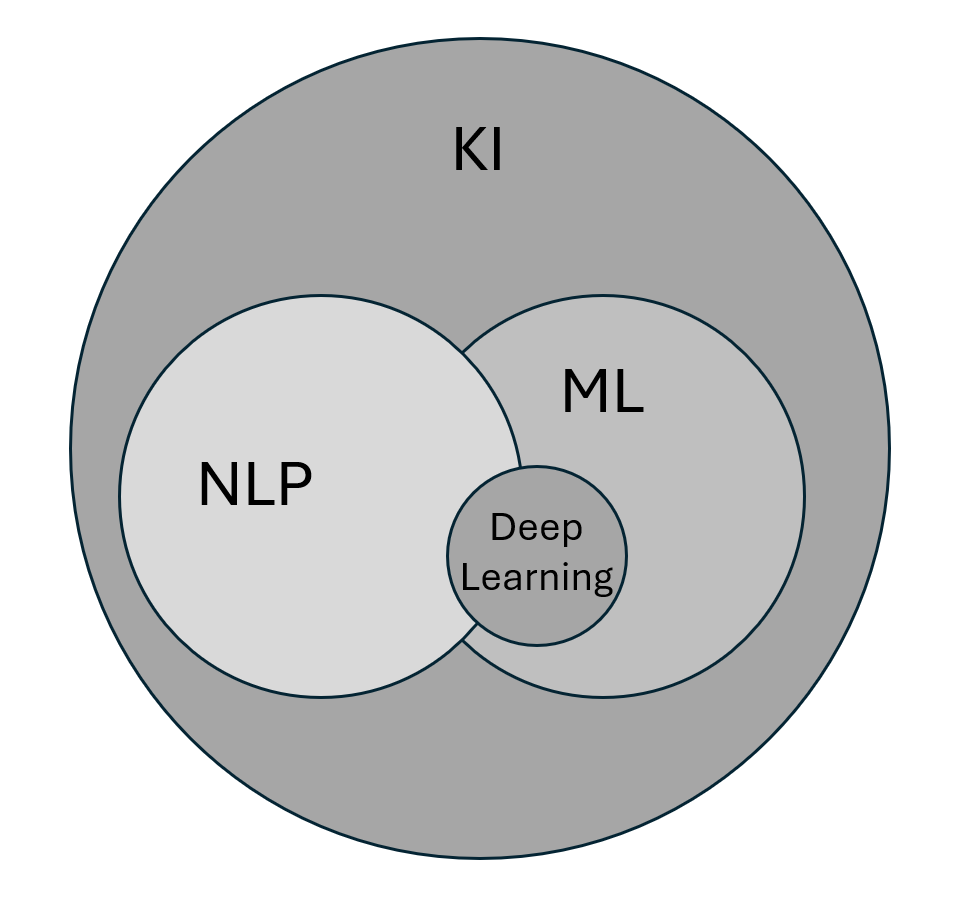
\includegraphics[width=0.6\textwidth]{img/KI_areas.png}
    \caption{Relevante Untergebiete der KI}
    \label{fig:areas_ki}
\end{figure}

Diese Technologien bilden die Grundlage für den Chatbot und ermöglichen es, Sprache zu verstehen und zu verarbeiten, um den Nutzern die gezielte und effiziente Suche nach Informationen zu erleichtern.


\section{Machine Learning und Deep Learning}

Ein wesentlicher Bestandteil der \ac{KI} ist das Machine Learning (\ac{ML}), welches es Systemen ermöglicht, Muster in großen Datenmengen zu erkennen, 
sich adaptiv zu verbessern und auf dieser Grundlage Prognosen oder Entscheidungen zu treffen. 
\ac{ML}-Modelle sind in der Lage, große Mengen an Textdaten zu verarbeiten und dabei Muster in der Sprache zu erlernen, die für die Erzeugung kohärenter und sinnvoller Antworten erforderlich sind.
Darüber hinaus ermöglicht es \ac{ML}, dass die Modelle durch kontinuierliche Interaktion mit Nutzern neue Daten aufnehmen und ihre Leistung im Laufe der Zeit optimieren. (\cite[S. 406]{Sarferaz2023})

Deep Learning ist eine spezialisierte Form des maschinellen Lernens, die auf tiefen neuronalen Netzwerken basiert. 
Diese tiefen neuronalen Netzwerke zeichnen sich durch mehrere versteckte Schichten aus, die es ermöglichen, komplexe Muster und Zusammenhänge zu erkennen. (\cite[S. 436 ff.]{LeCun2015})

In Kombination mit \ac{NLP} wird Deep Learning häufig in \ac{LLM}-Modellen eingesetzt, um tiefere semantische Strukturen und inhaltliche Verbindungen in Texten zu identifizieren. 
Durch die mehrschichtige Struktur neuronaler Netze kann Deep Learning daher die Erkennung komplexer Muster unterstützen und die Genauigkeit der vom Chatbot generierten Antworten erhöhen. (\cite[S. 605 f.]{Otter2021})


\section{Natural Language Processing}

Das Natural Language Processing (\ac{NLP}), ein spezialisiertes Teilgebiet der \ac{KI}, spielt ebenfalls eine wichtige unterstützende Rolle in dieser Arbeit. 
\ac{NLP} umfasst Techniken, die es Maschinen ermöglichen, menschliche Sprache nicht nur zu analysieren, sondern auch semantisch zu verstehen und zu generieren. (\cite[S. 31]{trapp2021})

Da der Chatbot in dieser Arbeit auf die effiziente Verarbeitung und Beantwortung von Anfragen in natürlicher Sprache ausgerichtet ist, 
unterstützt \ac{NLP} dabei, die in Dokumenten eingebetteten Informationen präzise zu extrahieren und in einer für den Nutzer verständlichen Form bereitzustellen. (\cite[S. 30]{Raj2019})

\section{Large Language Models}

Large Language Models (\acp{LLM}) sind eine Klasse von Deep Learning Modellen, die auf enorm großen Textkorpora trainiert werden, um eine Vielzahl von Sprachaufgaben zu bewältigen. 
Sie basieren in der Regel auf neuronalen Netzwerken, insbesondere auf transformatorbasierten Architekturen, die durch ihre Fähigkeit zur parallelen Verarbeitung und zur effizienten Nutzung von Kontextinformationen beeindrucken. (\cite[S. 7]{naveed2024})

Die Funktionsweise von \acp{LLM} beruht auf der Idee, dass Text als eine Sequenz von Wörtern oder Token betrachtet wird, wobei jedes Token mit dem vorherigen Kontext in Beziehung gesetzt wird (\cite[S. 4]{naveed2024}). 
Durch das Training auf Milliarden von Textbeispielen lernen die Modelle, Muster und Strukturen in der Sprache zu erkennen und basierend auf diesen Mustern Vorhersagen über die nächsten Token zu treffen. 
Je größer das Modell und je umfangreicher die Datenbasis, desto leistungsfähiger wird es in der Regel in Bezug auf das Verstehen und Generieren von Texten. (\cite[S. 1 ff.]{mielke2021})

Ein typisches \ac{LLM} ist so aufgebaut, dass es eine Vielzahl von Aufgaben wie das Verstehen von Kontext, das Beantworten von Fragen, das Verfassen von Texten oder sogar das Übersetzen von Sprachen bewältigen kann. 
Dabei greifen \acp{LLM} auf ihr internes Wissen zurück, das sie während des Trainings erworben haben, und sind in der Lage, eine Vielzahl von Aufgaben ohne spezialisierte Vorkenntnisse zu bewältigen. (\cite[S. 7]{Cerf2023})

\acp{LLM} wie GPT-4o und LLaMA3-70b basieren auf dieser Architektur und werden auf riesigen Datensätzen trainiert, die sie dazu befähigen, auf umfangreiche Sprachaufgaben zu reagieren (\cite[S. 782 f.]{Nowak2024}). 
Die in dieser Arbeit eingesetzten Modelle spielen eine zentrale Rolle, da sie die Grundlage für den Chatbot bilden, der entwickelt wird, um auf Basis von eingebetteten Dokumenten präzise und kontextbezogene Antworten zu generieren.

Ein entscheidender Vorteil von \acp{LLM} ist ihre Fähigkeit, auch komplexe Anfragen zu verstehen und im Kontext des gesamten Gesprächsverlaufes oder eines Dokumentenbestandes zu interpretieren. 
Die Verwendung von \ac{LLM} in Kombination mit \ac{RAG} verbessert zusätzlich die Fähigkeit des Chatbots, auf aktuelle und spezifische Informationen zuzugreifen (\cite[S. 1]{chen2023}). 

\section{Retrieval-Augmented Generation}

Retrieval-Augmented Generation (\ac{RAG}) ist ein fortschrittlicher Ansatz für \acp{LLM}, der für die Entwicklung von Chatbots relevant ist, die auf eingebetteten Dokumenten basieren. 
\ac{RAG} kombiniert \acp{LLM} mit einer Abrufkomponente, die es dem System ermöglicht, in Echtzeit externe Informationen aus einer Dokumentensammlung abzurufen anhanddessen eine Antwort zu generieren. 
Diese Methode erweist sich als besonders effizient, wenn präzise und aktuelle Informationen bereitgestellt werden sollen. (\cite[S. 1 ff.]{akkiraju2024factsbuildingretrievalaugmented}).

Im Rahmen dieser Arbeit wird \ac{RAG} verwendet, um sicherzustellen, dass der Chatbot nicht nur auf vortrainiertes Wissen zurückgreift, sondern auch spezifische Informationen aus eingebetteten Dokumenten bezieht. 
Dies ist besonders wichtig für die Freudenberg Gruppe, da der Chatbot auf unternehmensspezifische Dokumente zugreifen muss, um präzise Antworten zu generieren, die den Informationsbedarf der Mitarbeiter decken (\cite[S. 2]{akkiraju2024factsbuildingretrievalaugmented}).

Eine zentrale Technologie, die es dem Chatbot ermöglicht, diese Dokumente effizient zu durchsuchen und relevante Informationen zu extrahieren, ist das Embedding. 

\section{Embedding}

Embedding stellt eine grundlegende Technologie im \ac{RAG}-Prozess dar, die Wörter, Phrasen und ganze Dokumente in numerische Vektoren transformiert. 
Diese Vektoren repräsentieren semantische Beziehungen und ermöglichen es dem Chatbot, kontextuelle Zusammenhänge zwischen Textinhalten präzise zu identifizieren und relevante Informationen effizient zu extrahieren. (\cite[S. 1 ff.]{tennenholtz2024})

Wichtige Parameter im Embedding-Prozess sind die \textit{chunk size} und der \textit{top k}-Wert. Die \textit{chunk size} bezeichnet die Größe der Textabschnitte, in die ein Dokument aufgeteilt wird, 
bevor diese in Vektoren umgewandelt werden. Eine kleinere \textit{chunk size} ermöglicht eine feingranulare Analyse, während größere Chunks den Vorteil haben, umfassendere Zusammenhänge zu bewahren. 
Die Wahl der optimalen \textit{chunk size} ist entscheidend, um ein Gleichgewicht zwischen Detailgenauigkeit und Übersichtlichkeit der Informationen zu erreichen. (\cite[S. 1329 ff.]{Abdelazim2023})

Der \textit{top k}-Wert legt fest, wie viele der am höchsten bewerteten Chunks als Kontextinformationen an das \ac{LLM} weitergegeben werden (\cite{llamaindex}). Ein höherer \textit{top k}-Wert erhöht die Wahrscheinlichkeit, 
dass relevante Inhalte in den Kontext einfließen, kann jedoch die Präzision verringern, da mehr Informationen berücksichtigt werden. 
Diese Parameter tragen wesentlich dazu bei, die Effizienz und Genauigkeit des Chatbots zu optimieren, indem sie steuern, 
welche und wie viele Informationen aus den eingebetteten Dokumenten in die Antworten des Modells einfließen.

In dieser Arbeit sind Embeddings von zentraler Bedeutung, da der Chatbot die Fähigkeit benötigt, Dokumente semantisch zu analysieren und kontextbezogene Antworten auf Basis dieser Dokumente zu generieren. 
Ein Mitarbeiter der Freudenberg Gruppe kann somit neue Dokumente in das System hochladen, die der Chatbot bei zukünftigen Anfragen berücksichtigt. 
Durch die Einbettung dieser Dokumente in den Vektorraum ist der Chatbot in der Lage, die neuen Inhalte in seine Antworten zu integrieren, 
wodurch eine kontinuierliche Bereitstellung aktueller und relevanter Informationen sichergestellt wird (\cite[S. 4]{akkiraju2024factsbuildingretrievalaugmented}).

\section{Open Source}

Open Source bezeichnet Software, deren Quellcode öffentlich zugänglich ist und von jedem eingesehen, verändert und weiterverbreitet werden kann. 
Diese Offenheit ermöglicht es Entwicklern, die Software individuell anzupassen und weiterzuentwickeln, was einen hohen Grad an Flexibilität und Anpassbarkeit bietet. (\cite[S. 1]{Engelfried2010})
In bezug auf \ac{KI} bedeutet dies, dass Unternehmen \ac{LLM} nutzen können, ohne ihre Daten an externe Anbieter weitergeben zu müssen.

Für die Freudenberg Gruppe bietet die Nutzung von Open-Source-Lösungen signifikante Vorteile in Bezug auf Datenschutz und Datenhoheit. 
Durch die Implementierung in einer geschützten Umgebung wird sichergestellt, dass sensible Daten nicht an externe Anbieter wie Amazon oder Google übertragen werden müssen. 
Dies ist besonders wichtig, um strenge Datenschutzrichtlinien einzuhalten und die volle Kontrolle über die Daten zu behalten (\cite[S. 781 f.]{Nowak2024}).

Diese strategischen und technischen Überlegungen sind besonders wichtig für die Implementierung eines sicheren und datenschutzkonformen Chatbots, da sie es dem Unternehmen ermöglichen, 
sowohl die technische Infrastruktur als auch die Datensicherheit vollständig zu kontrollieren.

\section{SAP Business Technology Platform}

Die SAP Business Technology Platform (\ac{BTP}) ist eine umfassende cloudbasierte Plattform, die eine Vielzahl von Diensten bereitstellt, um Unternehmen bei der digitalen Transformation, 
Innovation und dem Wachstum zu unterstützen. Die \ac{BTP} umfasst zentrale Funktionen wie Anwendungsentwicklung, Integration, Datenmanagement, 
Analytik sowie Lösungen für Künstliche Intelligenz (\ac{KI}) und Maschinelles Lernen (\ac{ML}) (\cite[S. 103]{Gupta2024}). 

Zu den integrierten Lösungen gehören unter anderem SAP HANA, SAP Analytics Cloud, die SAP Intelligent Enterprise Suite sowie Enterprise AI. 
Diese Plattform ermöglicht es Unternehmen, ihre Geschäftsprozesse durch eine enge Integration und die Erweiterbarkeit der bereitgestellten Dienste zu optimieren und zu automatisieren. 
Die \ac{BTP} bietet sowohl vorgefertigte \ac{KI}-Anwendungen als auch die Möglichkeit, eigene, maßgeschneiderte Lösungen zu entwickeln und in die Unternehmensinfrastruktur zu integrieren. 
Mit der Einführung der \ac{BTP} im Jahr 2021, die die SAP Cloud Platform ersetzte, wurde eine intelligente Geschäftsmanagementplattform geschaffen, 
die die Kernfunktionalitäten von SAP S/4HANA umfasst und weltweite Echtzeit-Geschäftsoperationen ermöglicht. (\cite[S. 8 f.]{hrischevartificial}) 

Ein zentrales Element der \ac{BTP} ist die Cloud Foundry-Umgebung, die als Fundament der Plattform dient und eine cloudbasierte Laufzeitumgebung für die Entwicklung und Ausführung von Anwendungen bietet. 
Entwickler können hier Anwendungen in verschiedenen Programmiersprachen erstellen und bereitstellen, was der \ac{BTP} eine hohe Flexibilität verleiht. 
Die Cloud Foundry ist damit eine der Kernkomponenten der SAP \ac{BTP}, die es ermöglicht, cloud-native Anwendungen effizient zu betreiben. (\cite{sap2024cloudFoundry})

Für diese Arbeit ist die \ac{BTP} von besonderer Bedeutung, da sie die Grundlage für die Entwicklung und das Hosting des Chatbots darstellt. 
Insbesondere durch die flexible Nutzung der Cloud Foundry-Umgebung ermöglicht die \ac{BTP} es, die auf der Plattform verfügbaren \acp{LLM} effizient zu nutzen, 
um den Chatbot sicher und skalierbar in bestehende Geschäftsprozesse zu integrieren.

\section{SAP AI Core}

SAP AI Core bildet die zentrale Laufzeitumgebung für die Bereitstellung und das Management von Large Language Models (\acp{LLM}) und Embedding-Modellen auf der \ac{BTP} (\cite{sap2023aiCore}). 
Die Plattform stellt alle notwendigen Werkzeuge und eine flexible Infrastruktur bereit, um vortrainierte Modelle in produktiven Anwendungen einzusetzen und ihre Nutzung in Geschäftsprozesse zu integrieren. 
SAP AI Core ermöglicht diese Einbindung durch eine standardisierte \ac{API}-Schnittstelle, die eine direkte Integration in SAP-Anwendungen und bestehende Geschäftsanwendungen unterstützt. (\cite{sap2024aiCore})
Für die Entwicklung des Chatbots in dieser Arbeit ist SAP AI Core somit von zentraler Bedeutung, da es eine einfache Anbindung an die gewählten \acp{LLM} und die relevanten \ac{KI}-Funktionen bietet (\cite[S. 9]{hrischevartificial}).

Neben der Integration von SAP AI Core über die \ac{API}-Schnittstelle bietet SAP auch eine Python AI Core \ac{SDK}, die die Kommunikation und Interaktion mit den \acp{LLM} erheblich vereinfacht (\cite{sap2024aiCore}). 
Diese \ac{SDK} bietet leicht zugängliche Funktionen, um Prompts zu senden und Antworten zu empfangen, 
was die Implementierung von Retrieval-Augmented Generation (\ac{RAG}) in den Chatbot unterstützt und die Nutzung vortrainierter Modelle optimiert. 
So kann der Chatbot der Freudenberg Gruppe die benötigten Informationen auf Grundlage der eingebetteten Dokumente effizient bereitstellen, ohne die Notwendigkeit zusätzlicher Modelltrainings. (\cite{pythonAICoreSDK})

Mit SAP AI Core profitieren Anwender von einer verwalteten Umgebung, die alle notwendigen Abhängigkeiten integriert und somit den Aufwand für den Aufbau einer eigenen Modellinfrastruktur reduziert (\cite{sap2024aiCore}).
Dies schafft eine zuverlässige und einfach zu handhabende Umgebung für produktive \ac{KI}-Anwendungen und trägt dazu bei, \ac{KI}-Projekte schneller und kosteneffizienter in die Realität umzusetzen.

\section{LlamaIndex}

LlamaIndex ist eine zentrale Komponente zur Implementierung von Retrieval-Augmented Generation (\ac{RAG}) in Chatbots. 
Es ermöglicht eine effiziente semantische Suche innerhalb großer Dokumentbestände und erlaubt dem Chatbot, relevante Informationen in Echtzeit abzurufen und diese in die Antwortgenerierung zu integrieren (\cite{llamaindex}).

In der vorliegenden Arbeit wird LlamaIndex zur Entwicklung des Chatbots genutzt, indem es eine eine Similarity-Suche zwischen Benutzeranfragen und den eingebetteten Dokumenten durchführt und somit relevante Abschnitte identifiziert. 
Dies steigert die Relevanz und Genauigkeit der generierten Antworten und ermöglicht es den Mitarbeitern der Freudenberg Gruppe, schnell und präzise auf die benötigten Informationen zuzugreifen.